\documentclass[NEMO_book]{subfiles}
\begin{document}
% ================================================================
% Iso-neutral diffusion :
% ================================================================
\chapter[Iso-neutral diffusion and eddy advection using
triads]{Iso-neutral diffusion and eddy advection using triads}
\label{sec:triad}
\minitoc
\pagebreak
\section{Choice of \ngn{namtra\_ldf} namelist parameters}
%-----------------------------------------nam_traldf------------------------------------------------------
\namdisplay{namtra_ldf}
%---------------------------------------------------------------------------------------------------------
If the namelist variable \np{ln\_traldf\_grif} is set true (and
\key{ldfslp} is set), \NEMO updates both active and passive tracers
using the Griffies triad representation of iso-neutral diffusion and
the eddy-induced advective skew (GM) fluxes. Otherwise (by default) the
filtered version of Cox's original scheme is employed
(\S\ref{LDF_slp}). In the present implementation of the Griffies
scheme, the advective skew fluxes are implemented even if
\key{traldf\_eiv} is not set.

Values of iso-neutral diffusivity and GM coefficient are set as
described in \S\ref{LDF_coef}. If none of the keys \key{traldf\_cNd},
N=1,2,3 is set (the default), spatially constant iso-neutral $A_l$ and
GM diffusivity $A_e$ are directly set by \np{rn\_aeih\_0} and
\np{rn\_aeiv\_0}. If 2D-varying coefficients are set with
\key{traldf\_c2d} then $A_l$ is reduced in proportion with horizontal
scale factor according to \eqref{Eq_title} \footnote{Except in global ORCA
  $0.5^{\circ}$ runs with \key{traldf\_eiv}, where
  $A_l$ is set like $A_e$ but with a minimum vale of
  $100\;\mathrm{m}^2\;\mathrm{s}^{-1}$}. In idealised setups with
\key{traldf\_c2d}, $A_e$ is reduced similarly, but if \key{traldf\_eiv}
is set in the global configurations with \key{traldf\_c2d}, a horizontally varying $A_e$ is
instead set from the Held-Larichev parameterisation\footnote{In this
  case, $A_e$ at low latitudes $|\theta|<20^{\circ}$ is further
  reduced by a factor $|f/f_{20}|$, where $f_{20}$ is the value of $f$
  at $20^{\circ}$~N} (\mdl{ldfeiv}) and \np{rn\_aeiv\_0} is ignored
unless it is zero.

The options specific to the Griffies scheme include:
\begin{description}[font=\normalfont]
\item[\np{ln\_traldf\_gdia}] Default value is false. See \S\ref{sec:triad:sfdiag}. If this is set true, time-mean
  eddy-advective (GM) velocities are output for diagnostic purposes, even
  though the eddy advection is accomplished by means of the skew
  fluxes.
\item[\np{ln\_traldf\_iso}] See \S\ref{sec:triad:taper}. If this is set false (the default), then
  `iso-neutral' mixing is accomplished within the surface mixed-layer
  along slopes linearly decreasing with depth from the value immediately below
  the mixed-layer to zero (flat) at the surface (\S\ref{sec:triad:lintaper}). This is the same
  treatment as used in the default implementation
  \S\ref{LDF_slp_iso}; Fig.~\ref{Fig_eiv_slp}.  Where
  \np{ln\_traldf\_iso} is set true, the vertical skew flux is further
  reduced to ensure no vertical buoyancy flux, giving an almost pure
  horizontal diffusive tracer flux within the mixed layer. This is similar to
  the tapering suggested by \citet{Gerdes1991}. See \S\ref{sec:triad:Gerdes-taper}
\item[\np{ln\_traldf\_botmix}] See \S\ref{sec:triad:iso_bdry}. If this
  is set false (the default) then the lateral diffusive fluxes
  associated with triads partly masked by topography are neglected. If
  it is set true, however, then these lateral diffusive fluxes are
  applied, giving smoother bottom tracer fields at the cost of
  introducing diapycnal mixing.
\end{description}
\section{Triad formulation of iso-neutral diffusion}
\label{sec:triad:iso}
We have implemented into \NEMO a scheme inspired by \citet{Griffies_al_JPO98}, but formulated within the \NEMO
framework, using scale factors rather than grid-sizes.

\subsection{The iso-neutral diffusion operator}
The iso-neutral second order tracer diffusive operator for small
angles between iso-neutral surfaces and geopotentials is given by
\eqref{Eq_PE_iso_tensor}:
\begin{subequations} \label{eq:triad:PE_iso_tensor}
  \begin{equation}
    D^{lT}=-\Div\vect{f}^{lT}\equiv
    -\frac{1}{e_1e_2e_3}\left[\pd{i}\left (f_1^{lT}e_2e_3\right) +
      \pd{j}\left (f_2^{lT}e_2e_3\right) + \pd{k}\left (f_3^{lT}e_1e_2\right)\right],
  \end{equation}
  where the diffusive flux per unit area of physical space
  \begin{equation}
    \vect{f}^{lT}=-\Alt\Re\cdot\grad T,
  \end{equation}
  \begin{equation}
    \label{eq:triad:PE_iso_tensor:c}
    \mbox{with}\quad \;\;\Re =
    \begin{pmatrix}
      1&0&-r_1\mystrut \\
      0&1&-r_2\mystrut \\
      -r_1&-r_2&r_1 ^2+r_2 ^2\mystrut
    \end{pmatrix}
    \quad \text{and} \quad\grad T=
    \begin{pmatrix}
      \frac{1}{e_1}\pd[T]{i}\mystrut \\
      \frac{1}{e_2}\pd[T]{j}\mystrut \\
      \frac{1}{e_3}\pd[T]{k}\mystrut
    \end{pmatrix}.
  \end{equation}
\end{subequations}
% \left( {{\begin{array}{*{20}c}
%  1 \hfill & 0 \hfill & {-r_1 } \hfill \\
%  0 \hfill & 1 \hfill & {-r_2 } \hfill \\
%  {-r_1 } \hfill & {-r_2 } \hfill & {r_1 ^2+r_2 ^2} \hfill \\
% \end{array} }} \right)
 Here \eqref{Eq_PE_iso_slopes}
\begin{align*}
  r_1 &=-\frac{e_3 }{e_1 } \left( \frac{\partial \rho }{\partial i}
  \right)
  \left( {\frac{\partial \rho }{\partial k}} \right)^{-1} \\
  &=-\frac{e_3 }{e_1 } \left( -\alpha\frac{\partial T }{\partial i} +
    \beta\frac{\partial S }{\partial i} \right) \left(
    -\alpha\frac{\partial T }{\partial k} + \beta\frac{\partial S
    }{\partial k} \right)^{-1}
\end{align*}
is the $i$-component of the slope of the iso-neutral surface relative to the computational
surface, and $r_2$ is the $j$-component.

We will find it useful to consider the fluxes per unit area in $i,j,k$
space; we write
\begin{equation}
  \label{eq:triad:Fijk}
  \vect{F}_{\mathrm{iso}}=\left(f_1^{lT}e_2e_3, f_2^{lT}e_1e_3, f_3^{lT}e_1e_2\right).
\end{equation}
Additionally, we will sometimes write the contributions towards the
fluxes $\vect{f}$ and $\vect{F}_\mathrm{iso}$ from the component
$R_{ij}$ of $\Re$ as $f_{ij}$, $F_{\mathrm{iso}\: ij}$, with
$f_{ij}=R_{ij}e_i^{-1}\partial T/\partial x_i$ (no summation) etc.

The off-diagonal terms of the small angle diffusion tensor
\eqref{Eq_PE_iso_tensor}, \eqref{eq:triad:PE_iso_tensor:c} produce skew-fluxes along the
$i$- and $j$-directions resulting from the vertical tracer gradient:
\begin{align}
  \label{eq:triad:i13c}
  f_{13}=&+\Alt r_1\frac{1}{e_3}\frac{\partial T}{\partial k},\qquad f_{23}=+\Alt r_2\frac{1}{e_3}\frac{\partial T}{\partial k}\\
\intertext{and in the k-direction resulting from the lateral tracer gradients}
  \label{eq:triad:i31c}
 f_{31}+f_{32}=& \Alt r_1\frac{1}{e_1}\frac{\partial T}{\partial i}+\Alt r_2\frac{1}{e_1}\frac{\partial T}{\partial i}
\end{align}

The vertical diffusive flux associated with the $_{33}$
component of the small angle diffusion tensor is
\begin{equation}
  \label{eq:triad:i33c}
  f_{33}=-\Alt(r_1^2 +r_2^2) \frac{1}{e_3}\frac{\partial T}{\partial k}.
\end{equation}

Since there are no cross terms involving $r_1$ and $r_2$ in the above, we can
consider the iso-neutral diffusive fluxes separately in the $i$-$k$ and $j$-$k$
planes, just adding together the vertical components from each
plane. The following description will describe the fluxes on the $i$-$k$
plane.

There is no natural discretization for the $i$-component of the
skew-flux, \eqref{eq:triad:i13c}, as
although it must be evaluated at $u$-points, it involves vertical
gradients (both for the tracer and the slope $r_1$), defined at
$w$-points. Similarly, the vertical skew flux, \eqref{eq:triad:i31c}, is evaluated at
$w$-points but involves horizontal gradients defined at $u$-points.

\subsection{The standard discretization}
The straightforward approach to discretize the lateral skew flux
\eqref{eq:triad:i13c} from tracer cell $i,k$ to $i+1,k$, introduced in 1995
into OPA, \eqref{Eq_tra_ldf_iso}, is to calculate a mean vertical
gradient at the $u$-point from the average of the four surrounding
vertical tracer gradients, and multiply this by a mean slope at the
$u$-point, calculated from the averaged surrounding vertical density
gradients. The total area-integrated skew-flux (flux per unit area in
$ijk$ space) from tracer cell $i,k$
to $i+1,k$, noting that the $e_{{3}_{i+1/2}^k}$ in the area
$e{_{3}}_{i+1/2}^k{e_{2}}_{i+1/2}i^k$ at the $u$-point cancels out with
the $1/{e_{3}}_{i+1/2}^k$ associated with the vertical tracer
gradient, is then \eqref{Eq_tra_ldf_iso}
\begin{equation*}
  \left(F_u^{13} \right)_{i+\hhalf}^k = \Alts_{i+\hhalf}^k
  {e_{2}}_{i+1/2}^k \overline{\overline
    r_1} ^{\,i,k}\,\overline{\overline{\delta_k T}}^{\,i,k},
\end{equation*}
where
\begin{equation*}
  \overline{\overline
   r_1} ^{\,i,k} = -\frac{{e_{3u}}_{i+1/2}^k}{{e_{1u}}_{i+1/2}^k}
  \frac{\delta_{i+1/2} [\rho]}{\overline{\overline{\delta_k \rho}}^{\,i,k}},
\end{equation*}
and here and in the following we drop the $^{lT}$ superscript from
$\Alt$ for simplicity.
Unfortunately the resulting combination $\overline{\overline{\delta_k
    \bullet}}^{\,i,k}$ of a $k$ average and a $k$ difference %of the tracer
reduces to $\bullet_{k+1}-\bullet_{k-1}$, so two-grid-point oscillations are
invisible to this discretization of the iso-neutral operator. These
\emph{computational modes} will not be damped by this operator, and
may even possibly be amplified by it.  Consequently, applying this
operator to a tracer does not guarantee the decrease of its
global-average variance. To correct this, we introduced a smoothing of
the slopes of the iso-neutral surfaces (see \S\ref{LDF}). This
technique works for $T$ and $S$ in so far as they are active tracers
($i.e.$ they enter the computation of density), but it does not work
for a passive tracer.
\subsection{Expression of the skew-flux in terms of triad slopes}
\citep{Griffies_al_JPO98} introduce a different discretization of the
off-diagonal terms that nicely solves the problem.
% Instead of multiplying the mean slope calculated at the $u$-point by
% the mean vertical gradient at the $u$-point,
% >>>>>>>>>>>>>>>>>>>>>>>>>>>>
\begin{figure}[h] \begin{center}
    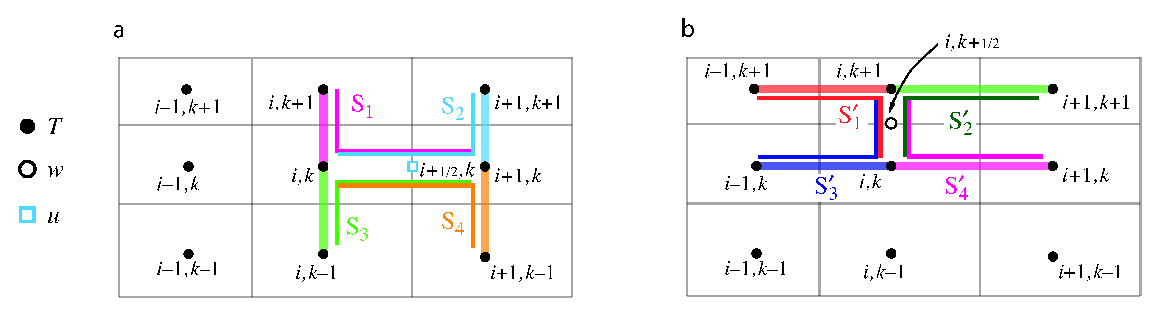
\includegraphics[width=1.05\textwidth]{Fig_GRIFF_triad_fluxes}
    \caption{ \label{fig:triad:ISO_triad}
      (a) Arrangement of triads $S_i$ and tracer gradients to
           give lateral tracer flux from box $i,k$ to $i+1,k$
      (b) Triads $S'_i$ and tracer gradients to give vertical tracer flux from
            box $i,k$ to $i,k+1$.}
 \end{center} \end{figure}
% >>>>>>>>>>>>>>>>>>>>>>>>>>>>
They get the skew flux from the products of the vertical gradients at
each $w$-point surrounding the $u$-point with the corresponding `triad'
slope calculated from the lateral density gradient across the $u$-point
divided by the vertical density gradient at the same $w$-point as the
tracer gradient. See Fig.~\ref{fig:triad:ISO_triad}a, where the thick lines
denote the tracer gradients, and the thin lines the corresponding
triads, with slopes $s_1, \dotsc s_4$. The total area-integrated
skew-flux from tracer cell $i,k$ to $i+1,k$
\begin{multline}
  \label{eq:triad:i13}
  \left( F_u^{13}  \right)_{i+\frac{1}{2}}^k = \Alts_{i+1}^k a_1 s_1
  \delta _{k+\frac{1}{2}} \left[ T^{i+1}
  \right]/e_{{3w}_{i+1}}^{k+\frac{1}{2}}  + \Alts _i^k a_2 s_2 \delta
  _{k+\frac{1}{2}} \left[ T^i
  \right]/e_{{3w}_{i+1}}^{k+\frac{1}{2}} \\
   +\Alts _{i+1}^k a_3 s_3 \delta _{k-\frac{1}{2}} \left[ T^{i+1}
  \right]/e_{{3w}_{i+1}}^{k+\frac{1}{2}}  +\Alts _i^k a_4 s_4 \delta
  _{k-\frac{1}{2}} \left[ T^i \right]/e_{{3w}_{i+1}}^{k+\frac{1}{2}},
\end{multline}
where the contributions of the triad fluxes are weighted by areas
$a_1, \dotsc a_4$, and $\Alts$ is now defined at the tracer points
rather than the $u$-points. This discretization gives a much closer
stencil, and disallows the two-point computational modes.

 The vertical skew flux \eqref{eq:triad:i31c} from tracer cell $i,k$ to $i,k+1$ at the
$w$-point $i,k+\hhalf$ is constructed similarly (Fig.~\ref{fig:triad:ISO_triad}b)
by multiplying lateral tracer gradients from each of the four
surrounding $u$-points by the appropriate triad slope:
\begin{multline}
  \label{eq:triad:i31}
  \left( F_w^{31} \right) _i ^{k+\frac{1}{2}} =  \Alts_i^{k+1} a_{1}'
  s_{1}' \delta _{i-\frac{1}{2}} \left[ T^{k+1} \right]/{e_{3u}}_{i-\frac{1}{2}}^{k+1}
   +\Alts_i^{k+1} a_{2}' s_{2}' \delta _{i+\frac{1}{2}} \left[ T^{k+1} \right]/{e_{3u}}_{i+\frac{1}{2}}^{k+1}\\
  + \Alts_i^k a_{3}' s_{3}' \delta _{i-\frac{1}{2}} \left[ T^k\right]/{e_{3u}}_{i-\frac{1}{2}}^k
  +\Alts_i^k a_{4}' s_{4}' \delta _{i+\frac{1}{2}} \left[ T^k \right]/{e_{3u}}_{i+\frac{1}{2}}^k.
\end{multline}

We notate the triad slopes $s_i$ and $s'_i$ in terms of the `anchor point' $i,k$
(appearing in both the vertical and lateral gradient), and the $u$- and
$w$-points $(i+i_p,k)$, $(i,k+k_p)$ at the centres of the `arms' of the
triad as follows (see also Fig.~\ref{fig:triad:ISO_triad}):
\begin{equation}
  \label{eq:triad:R}
  _i^k \mathbb{R}_{i_p}^{k_p}
  =-\frac{ {e_{3w}}_{\,i}^{\,k+k_p}} { {e_{1u}}_{\,i+i_p}^{\,k}}
  \
  \frac
  {\left(\alpha / \beta \right)_i^k  \ \delta_{i + i_p}[T^k] - \delta_{i + i_p}[S^k] }
  {\left(\alpha / \beta \right)_i^k  \ \delta_{k+k_p}[T^i ] - \delta_{k+k_p}[S^i ] }.
\end{equation}
In calculating the slopes of the local neutral
surfaces, the expansion coefficients $\alpha$ and $\beta$ are
evaluated at the anchor points of the triad \footnote{Note that in \eqref{eq:triad:R} we use the ratio $\alpha / \beta$
instead of multiplying the temperature derivative by $\alpha$ and the
salinity derivative by $\beta$. This is more efficient as the ratio
$\alpha / \beta$ can to be evaluated directly}, while the metrics are
calculated at the $u$- and $w$-points on the arms.

% >>>>>>>>>>>>>>>>>>>>>>>>>>>>
\begin{figure}[h] \begin{center}
    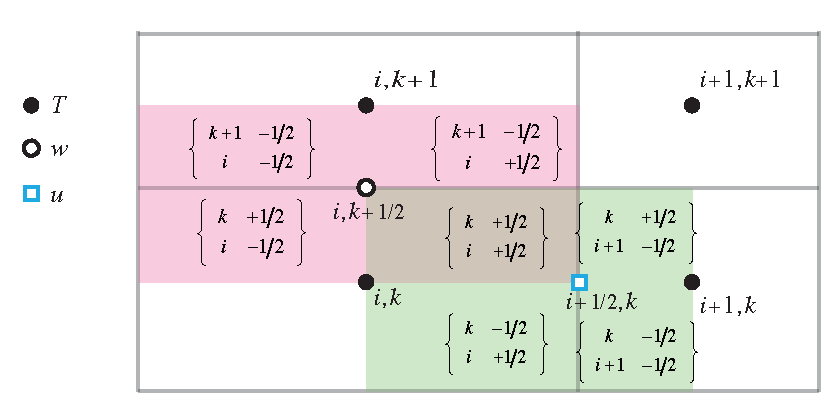
\includegraphics[width=0.80\textwidth]{Fig_GRIFF_qcells}
    \caption{   \label{fig:triad:qcells}
    Triad notation for quarter cells. $T$-cells are inside
      boxes, while the  $i+\half,k$ $u$-cell is shaded in green and the
      $i,k+\half$ $w$-cell is shaded in pink.}
  \end{center} \end{figure}
% >>>>>>>>>>>>>>>>>>>>>>>>>>>>

Each triad $\{_i^k\:_{i_p}^{k_p}\}$ is associated (Fig.~\ref{fig:triad:qcells}) with the quarter
cell that is the intersection of the $i,k$ $T$-cell, the $i+i_p,k$
$u$-cell and the $i,k+k_p$ $w$-cell. Expressing the slopes $s_i$ and
$s'_i$ in \eqref{eq:triad:i13} and \eqref{eq:triad:i31} in this notation, we have
e.g.\ $s_1=s'_1={\:}_i^k \mathbb{R}_{1/2}^{1/2}$. Each triad slope $_i^k
\mathbb{R}_{i_p}^{k_p}$ is used once (as an $s$) to calculate the
lateral flux along its $u$-arm, at $(i+i_p,k)$, and then again as an
$s'$ to calculate the vertical flux along its $w$-arm at
$(i,k+k_p)$. Each vertical area $a_i$ used to calculate the lateral
flux and horizontal area $a'_i$ used to calculate the vertical flux
can also be identified as the area across the $u$- and $w$-arms of a
unique triad, and we notate these areas, similarly to the triad
slopes, as $_i^k{\mathbb{A}_u}_{i_p}^{k_p}$,
$_i^k{\mathbb{A}_w}_{i_p}^{k_p}$, where e.g. in \eqref{eq:triad:i13}
$a_{1}={\:}_i^k{\mathbb{A}_u}_{1/2}^{1/2}$, and in \eqref{eq:triad:i31}
$a'_{1}={\:}_i^k{\mathbb{A}_w}_{1/2}^{1/2}$.

\subsection{The full triad fluxes}
A key property of iso-neutral diffusion is that it should not affect
the (locally referenced) density. In particular there should be no
lateral or vertical density flux. The lateral density flux disappears so long as the
area-integrated lateral diffusive flux from tracer cell $i,k$ to
$i+1,k$ coming from the $_{11}$ term of the diffusion tensor takes the
form
\begin{equation}
  \label{eq:triad:i11}
  \left( F_u^{11} \right) _{i+\frac{1}{2}} ^{k} =
  - \left( \Alts_i^{k+1} a_{1} + \Alts_i^{k+1} a_{2} + \Alts_i^k
    a_{3} + \Alts_i^k a_{4} \right)
  \frac{\delta _{i+1/2} \left[ T^k\right]}{{e_{1u}}_{\,i+1/2}^{\,k}},
\end{equation}
where the areas $a_i$ are as in \eqref{eq:triad:i13}. In this case,
separating the total lateral flux, the sum of \eqref{eq:triad:i13} and
\eqref{eq:triad:i11}, into triad components, a lateral tracer
flux
\begin{equation}
  \label{eq:triad:latflux-triad}
  _i^k {\mathbb{F}_u}_{i_p}^{k_p} (T) = - \Alts_i^k{ \:}_i^k{\mathbb{A}_u}_{i_p}^{k_p}
  \left(
    \frac{ \delta_{i+ i_p}[T^k] }{ {e_{1u}}_{\,i + i_p}^{\,k} }
    -\ {_i^k\mathbb{R}_{i_p}^{k_p}} \
    \frac{ \delta_{k+k_p} [T^i] }{{e_{3w}}_{\,i}^{\,k+k_p} }
  \right)
\end{equation}
can be identified with each triad. Then, because the
same metric factors ${e_{3w}}_{\,i}^{\,k+k_p}$ and
${e_{1u}}_{\,i+i_p}^{\,k}$ are employed for both the density gradients
in $ _i^k \mathbb{R}_{i_p}^{k_p}$ and the tracer gradients, the lateral
density flux associated with each triad separately disappears.
\begin{equation}
  \label{eq:triad:latflux-rho}
  {\mathbb{F}_u}_{i_p}^{k_p} (\rho)=-\alpha _i^k {\:}_i^k {\mathbb{F}_u}_{i_p}^{k_p} (T) + \beta_i^k {\:}_i^k {\mathbb{F}_u}_{i_p}^{k_p} (S)=0
\end{equation}
Thus the total flux $\left( F_u^{31} \right) ^i _{i,k+\frac{1}{2}} +
\left( F_u^{11} \right) ^i _{i,k+\frac{1}{2}}$ from tracer cell $i,k$
to $i+1,k$ must also vanish since it is a sum of four such triad fluxes.

The squared slope $r_1^2$ in the expression \eqref{eq:triad:i33c} for the
$_{33}$ component is also expressed in terms of area-weighted
squared triad slopes, so the area-integrated vertical flux from tracer
cell $i,k$ to $i,k+1$ resulting from the $r_1^2$ term is
\begin{equation}
  \label{eq:triad:i33}
  \left( F_w^{33} \right) _i^{k+\frac{1}{2}} =
    - \left( \Alts_i^{k+1} a_{1}' s_{1}'^2
    + \Alts_i^{k+1} a_{2}' s_{2}'^2
    + \Alts_i^k a_{3}' s_{3}'^2
    + \Alts_i^k a_{4}' s_{4}'^2 \right)\delta_{k+\frac{1}{2}} \left[ T^{i+1} \right],
\end{equation}
where the areas $a'$ and slopes $s'$ are the same as in
\eqref{eq:triad:i31}.
Then, separating the total vertical flux, the sum of \eqref{eq:triad:i31} and
\eqref{eq:triad:i33}, into triad components,  a vertical flux
\begin{align}
  \label{eq:triad:vertflux-triad}
  _i^k {\mathbb{F}_w}_{i_p}^{k_p} (T)
  &= \Alts_i^k{\: }_i^k{\mathbb{A}_w}_{i_p}^{k_p}
  \left(
    {_i^k\mathbb{R}_{i_p}^{k_p}}\frac{ \delta_{i+ i_p}[T^k] }{ {e_{1u}}_{\,i + i_p}^{\,k} }
    -\ \left({_i^k\mathbb{R}_{i_p}^{k_p}}\right)^2 \
    \frac{ \delta_{k+k_p} [T^i] }{{e_{3w}}_{\,i}^{\,k+k_p} }
  \right) \\
  &= - \left(\left.{ }_i^k{\mathbb{A}_w}_{i_p}^{k_p}\right/{ }_i^k{\mathbb{A}_u}_{i_p}^{k_p}\right)
   {_i^k\mathbb{R}_{i_p}^{k_p}}{\: }_i^k{\mathbb{F}_u}_{i_p}^{k_p} (T) \label{eq:triad:vertflux-triad2}
\end{align}
may be associated with each triad. Each vertical density flux $_i^k {\mathbb{F}_w}_{i_p}^{k_p} (\rho)$
associated with a triad then separately disappears (because the
lateral flux $_i^k{\mathbb{F}_u}_{i_p}^{k_p} (\rho)$
disappears). Consequently the total vertical density flux $\left( F_w^{31} \right)_i ^{k+\frac{1}{2}} +
\left( F_w^{33} \right)_i^{k+\frac{1}{2}}$ from tracer cell $i,k$
to $i,k+1$ must also vanish since it is a sum of four such triad
fluxes.

We can explicitly identify (Fig.~\ref{fig:triad:qcells}) the triads associated with the $s_i$, $a_i$, and $s'_i$, $a'_i$ used in the definition of
the $u$-fluxes and $w$-fluxes in
\eqref{eq:triad:i31}, \eqref{eq:triad:i13}, \eqref{eq:triad:i11} \eqref{eq:triad:i33} and
Fig.~\ref{fig:triad:ISO_triad} to  write out the iso-neutral fluxes at $u$- and
$w$-points as sums of the triad fluxes that cross the $u$- and $w$-faces:
%(Fig.~\ref{Fig_ISO_triad}):
\begin{flalign} \label{Eq_iso_flux} \vect{F}_\mathrm{iso}(T) &\equiv
  \sum_{\substack{i_p,\,k_p}}
  \begin{pmatrix}
    {_{i+1/2-i_p}^k {\mathbb{F}_u}_{i_p}^{k_p} } (T)      \\
    \\
    {_i^{k+1/2-k_p} {\mathbb{F}_w}_{i_p}^{k_p} } (T)      \\
  \end{pmatrix}.
\end{flalign}
\subsection{Ensuring the scheme does not increase tracer variance}
\label{sec:triad:variance}

We now require that this operator should not increase the
globally-integrated tracer variance.
%This changes according to
% \begin{align*}
% &\int_D  D_l^T \; T \;dv \equiv  \sum_{i,k} \left\{ T \ D_l^T \ b_T \right\}    \\
% &\equiv + \sum_{i,k} \sum_{\substack{i_p,\,k_p}} \left\{
% 		\delta_{i} \left[{_{i+1/2-i_p}^k {\mathbb{F}_u }_{i_p}^{k_p}} \right]
% 	     + \delta_{k} \left[ {_i^{k+1/2-k_p} {\mathbb{F}_w}_{i_p}^{k_p}} \right]  \ T \right\}    \\
% &\equiv  - \sum_{i,k} \sum_{\substack{i_p,\,k_p}} \left\{
%                 {_{i+1/2-i_p}^k {\mathbb{F}_u }_{i_p}^{k_p}} \ \delta_{i+1/2} [T]
%              + {_i^{k+1/2-k_p} {\mathbb{F}_w}_{i_p}^{k_p}}  \ \delta_{k+1/2} [T]   \right\}      \\
% \end{align*}
Each triad slope $_i^k\mathbb{R}_{i_p}^{k_p}$ drives a lateral flux
$_i^k{\mathbb{F}_u}_{i_p}^{k_p} (T)$ across the $u$-point $i+i_p,k$ and
a vertical flux $_i^k{\mathbb{F}_w}_{i_p}^{k_p} (T)$ across the
$w$-point $i,k+k_p$.  The lateral flux drives a net rate of change of
variance, summed over the two $T$-points $i+i_p-\half,k$ and $i+i_p+\half,k$, of
\begin{multline}
  {b_T}_{i+i_p-1/2}^k\left(\frac{\partial T}{\partial t}T\right)_{i+i_p-1/2}^k+
  \quad {b_T}_{i+i_p+1/2}^k\left(\frac{\partial T}{\partial
      t}T\right)_{i+i_p+1/2}^k \\
 \begin{split}
  &= -T_{i+i_p-1/2}^k{\;} _i^k{\mathbb{F}_u}_{i_p}^{k_p} (T) \quad + \quad  T_{i+i_p+1/2}^k
  {\;}_i^k{\mathbb{F}_u}_{i_p}^{k_p} (T) \\
  &={\;} _i^k{\mathbb{F}_u}_{i_p}^{k_p} (T)\,\delta_{i+ i_p}[T^k], \label{eq:triad:dvar_iso_i}
 \end{split}
\end{multline}
while the vertical flux similarly drives a net rate of change of
variance summed over the $T$-points $i,k+k_p-\half$ (above) and
$i,k+k_p+\half$ (below) of
\begin{equation}
\label{eq:triad:dvar_iso_k}
  _i^k{\mathbb{F}_w}_{i_p}^{k_p} (T) \,\delta_{k+ k_p}[T^i].
\end{equation}
The total variance tendency driven by the triad is the sum of these
two. Expanding $_i^k{\mathbb{F}_u}_{i_p}^{k_p} (T)$ and
$_i^k{\mathbb{F}_w}_{i_p}^{k_p} (T)$ with \eqref{eq:triad:latflux-triad} and
\eqref{eq:triad:vertflux-triad}, it is
\begin{multline*}
-\Alts_i^k\left \{
{ } _i^k{\mathbb{A}_u}_{i_p}^{k_p}
  \left(
    \frac{ \delta_{i+ i_p}[T^k] }{ {e_{1u}}_{\,i + i_p}^{\,k} }
    - {_i^k\mathbb{R}_{i_p}^{k_p}} \
    \frac{ \delta_{k+k_p} [T^i] }{{e_{3w}}_{\,i}^{\,k+k_p} }\right)\,\delta_{i+ i_p}[T^k] \right.\\
- \left. { } _i^k{\mathbb{A}_w}_{i_p}^{k_p}
  \left(
    \frac{ \delta_{i+ i_p}[T^k] }{ {e_{1u}}_{\,i + i_p}^{\,k} }
    -{\:}_i^k\mathbb{R}_{i_p}^{k_p}
    \frac{ \delta_{k+k_p} [T^i] }{{e_{3w}}_{\,i}^{\,k+k_p} }
  \right) {\,}_i^k\mathbb{R}_{i_p}^{k_p}\delta_{k+ k_p}[T^i]
\right \}.
\end{multline*}
The key point is then that if we require
$_i^k{\mathbb{A}_u}_{i_p}^{k_p}$ and $_i^k{\mathbb{A}_w}_{i_p}^{k_p}$
to be related to a triad volume $_i^k\mathbb{V}_{i_p}^{k_p}$ by
\begin{equation}
  \label{eq:triad:V-A}
  _i^k\mathbb{V}_{i_p}^{k_p}
  ={\;}_i^k{\mathbb{A}_u}_{i_p}^{k_p}\,{e_{1u}}_{\,i + i_p}^{\,k}
  ={\;}_i^k{\mathbb{A}_w}_{i_p}^{k_p}\,{e_{3w}}_{\,i}^{\,k + k_p},
\end{equation}
the variance tendency reduces to the perfect square
\begin{equation}
  \label{eq:triad:perfect-square}
  -\Alts_i^k{\:} _i^k\mathbb{V}_{i_p}^{k_p}
  \left(
    \frac{ \delta_{i+ i_p}[T^k] }{ {e_{1u}}_{\,i + i_p}^{\,k} }
    -{\:}_i^k\mathbb{R}_{i_p}^{k_p}
    \frac{ \delta_{k+k_p} [T^i] }{{e_{3w}}_{\,i}^{\,k+k_p} }
  \right)^2\leq 0.
\end{equation}
Thus, the constraint \eqref{eq:triad:V-A} ensures that the fluxes (\ref{eq:triad:latflux-triad}, \ref{eq:triad:vertflux-triad}) associated
with a given slope triad $_i^k\mathbb{R}_{i_p}^{k_p}$ do not increase
the net variance. Since the total fluxes are sums of such fluxes from
the various triads, this constraint, applied to all triads, is
sufficient to ensure that the globally integrated variance does not
increase.

The expression \eqref{eq:triad:V-A} can be interpreted as a discretization
of the global integral
\begin{equation}
  \label{eq:triad:cts-var}
  \frac{\partial}{\partial t}\int\!\half T^2\, dV =
  \int\!\mathbf{F}\cdot\nabla T\, dV,
\end{equation}
where, within each triad volume $_i^k\mathbb{V}_{i_p}^{k_p}$, the
lateral and vertical fluxes/unit area
\[
\mathbf{F}=\left(
\left.{}_i^k{\mathbb{F}_u}_{i_p}^{k_p} (T)\right/{}_i^k{\mathbb{A}_u}_{i_p}^{k_p},
\left.{\:}_i^k{\mathbb{F}_w}_{i_p}^{k_p} (T)\right/{}_i^k{\mathbb{A}_w}_{i_p}^{k_p}
 \right)
\]
and the gradient
 \[\nabla T = \left(
\left.\delta_{i+ i_p}[T^k] \right/ {e_{1u}}_{\,i + i_p}^{\,k},
\left.\delta_{k+ k_p}[T^i] \right/ {e_{3w}}_{\,i}^{\,k + k_p}
\right)
\]
\subsection{Triad volumes in Griffes's scheme and in \NEMO}
To complete the discretization we now need only specify the triad
volumes $_i^k\mathbb{V}_{i_p}^{k_p}$. \citet{Griffies_al_JPO98} identify
these $_i^k\mathbb{V}_{i_p}^{k_p}$ as the volumes of the quarter
cells, defined in terms of the distances between $T$, $u$,$f$ and
$w$-points. This is the natural discretization of
\eqref{eq:triad:cts-var}. The \NEMO model, however, operates with scale
factors instead of grid sizes, and scale factors for the quarter
cells are not defined. Instead, therefore we simply choose
\begin{equation}
  \label{eq:triad:V-NEMO}
  _i^k\mathbb{V}_{i_p}^{k_p}=\quarter {b_u}_{i+i_p}^k,
\end{equation}
as a quarter of the volume of the $u$-cell inside which the triad
quarter-cell lies. This has the nice property that when the slopes
$\mathbb{R}$ vanish, the lateral flux from tracer cell $i,k$ to
$i+1,k$ reduces to the classical form
\begin{equation}
  \label{eq:triad:lat-normal}
-\overline\Alts_{\,i+1/2}^k\;
\frac{{b_u}_{i+1/2}^k}{{e_{1u}}_{\,i + i_p}^{\,k}}
\;\frac{\delta_{i+ 1/2}[T^k] }{{e_{1u}}_{\,i + i_p}^{\,k}}
 = -\overline\Alts_{\,i+1/2}^k\;\frac{{e_{1w}}_{\,i + 1/2}^{\,k}\:{e_{1v}}_{\,i + 1/2}^{\,k}\;\delta_{i+ 1/2}[T^k]}{{e_{1u}}_{\,i + 1/2}^{\,k}}.
\end{equation}
In fact if the diffusive coefficient is defined at $u$-points, so that
we employ $\Alts_{i+i_p}^k$ instead of  $\Alts_i^k$ in the definitions of the
triad fluxes \eqref{eq:triad:latflux-triad} and \eqref{eq:triad:vertflux-triad},
we can replace $\overline{A}_{\,i+1/2}^k$ by $A_{i+1/2}^k$ in the above.

\subsection{Summary of the scheme}
The iso-neutral fluxes at $u$- and
$w$-points are the sums of the triad fluxes that cross the $u$- and
$w$-faces \eqref{Eq_iso_flux}:
\begin{subequations}\label{eq:triad:alltriadflux}
  \begin{flalign}\label{eq:triad:vect_isoflux}
    \vect{F}_\mathrm{iso}(T) &\equiv
    \sum_{\substack{i_p,\,k_p}}
    \begin{pmatrix}
      {_{i+1/2-i_p}^k {\mathbb{F}_u}_{i_p}^{k_p} } (T)      \\
      \\
      {_i^{k+1/2-k_p} {\mathbb{F}_w}_{i_p}^{k_p} } (T) 
    \end{pmatrix},
  \end{flalign}
  where \eqref{eq:triad:latflux-triad}:
  \begin{align}
    \label{eq:triad:triadfluxu}
    _i^k {\mathbb{F}_u}_{i_p}^{k_p} (T) &= - \Alts_i^k{
      \:}\frac{{{}_i^k\mathbb{V}}_{i_p}^{k_p}}{{e_{1u}}_{\,i + i_p}^{\,k}}
    \left(
      \frac{ \delta_{i+ i_p}[T^k] }{ {e_{1u}}_{\,i + i_p}^{\,k} }
      -\ {_i^k\mathbb{R}_{i_p}^{k_p}} \
      \frac{ \delta_{k+k_p} [T^i] }{{e_{3w}}_{\,i}^{\,k+k_p} }
    \right),\\
    \intertext{and}
    _i^k {\mathbb{F}_w}_{i_p}^{k_p} (T)
    &= \Alts_i^k{\: }\frac{{{}_i^k\mathbb{V}}_{i_p}^{k_p}}{{e_{3w}}_{\,i}^{\,k+k_p}}
    \left(
      {_i^k\mathbb{R}_{i_p}^{k_p}}\frac{ \delta_{i+ i_p}[T^k] }{ {e_{1u}}_{\,i + i_p}^{\,k} }
      -\ \left({_i^k\mathbb{R}_{i_p}^{k_p}}\right)^2 \
      \frac{ \delta_{k+k_p} [T^i] }{{e_{3w}}_{\,i}^{\,k+k_p} }
    \right),\label{eq:triad:triadfluxw}
  \end{align}
  with \eqref{eq:triad:V-NEMO}
  \begin{equation}
    \label{eq:triad:V-NEMO2}
    _i^k{\mathbb{V}}_{i_p}^{k_p}=\quarter {b_u}_{i+i_p}^k.
  \end{equation}
\end{subequations}

 The divergence of the expression \eqref{Eq_iso_flux} for the fluxes gives the iso-neutral diffusion tendency at
each tracer point:
\begin{equation} \label{eq:triad:iso_operator} D_l^T = \frac{1}{b_T}
  \sum_{\substack{i_p,\,k_p}} \left\{ \delta_{i} \left[{_{i+1/2-i_p}^k
        {\mathbb{F}_u }_{i_p}^{k_p}} \right] + \delta_{k} \left[
      {_i^{k+1/2-k_p} {\mathbb{F}_w}_{i_p}^{k_p}} \right] \right\}
\end{equation}
where $b_T= e_{1T}\,e_{2T}\,e_{3T}$ is the volume of $T$-cells.
The diffusion scheme satisfies the following six properties:
\begin{description}
\item[$\bullet$ horizontal diffusion] The discretization of the
  diffusion operator recovers \eqref{eq:triad:lat-normal} the traditional five-point Laplacian in
  the limit of flat iso-neutral direction :
  \begin{equation} \label{eq:triad:iso_property0} D_l^T = \frac{1}{b_T} \
    \delta_{i} \left[ \frac{e_{2u}\,e_{3u}}{e_{1u}} \;
      \overline\Alts^{\,i} \; \delta_{i+1/2}[T] \right] \qquad
    \text{when} \quad { _i^k \mathbb{R}_{i_p}^{k_p} }=0
  \end{equation}

\item[$\bullet$ implicit treatment in the vertical] Only tracer values
  associated with a single water column appear in the expression
  \eqref{eq:triad:i33} for the $_{33}$ fluxes, vertical fluxes driven by
  vertical gradients. This is of paramount importance since it means
  that a time-implicit algorithm can be used to solve the vertical
  diffusion equation. This is necessary
 since the vertical eddy
  diffusivity associated with this term,
  \begin{equation}
    \frac{1}{b_w}\sum_{\substack{i_p, \,k_p}} \left\{
      {\:}_i^k\mathbb{V}_{i_p}^{k_p} \: \Alts_i^k \: \left(_i^k \mathbb{R}_{i_p}^{k_p}\right)^2
    \right\}  =
    \frac{1}{4b_w}\sum_{\substack{i_p, \,k_p}} \left\{
      {b_u}_{i+i_p}^k\: \Alts_i^k \: \left(_i^k \mathbb{R}_{i_p}^{k_p}\right)^2
    \right\},
 \end{equation}
  (where $b_w= e_{1w}\,e_{2w}\,e_{3w}$ is the volume of $w$-cells) can be quite large.

\item[$\bullet$ pure iso-neutral operator] The iso-neutral flux of
  locally referenced potential density is zero. See
  \eqref{eq:triad:latflux-rho} and \eqref{eq:triad:vertflux-triad2}.

\item[$\bullet$ conservation of tracer] The iso-neutral diffusion
  conserves tracer content, $i.e.$
  \begin{equation} \label{eq:triad:iso_property1} \sum_{i,j,k} \left\{ D_l^T \
      b_T \right\} = 0
  \end{equation}
  This property is trivially satisfied since the iso-neutral diffusive
  operator is written in flux form.

\item[$\bullet$ no increase of tracer variance] The iso-neutral diffusion
  does not increase the tracer variance, $i.e.$
  \begin{equation} \label{eq:triad:iso_property2} \sum_{i,j,k} \left\{ T \ D_l^T
      \ b_T \right\} \leq 0
  \end{equation}
  The property is demonstrated in
  \S\ref{sec:triad:variance} above. It is a key property for a diffusion
  term. It means that it is also a dissipation term, $i.e.$ it
  dissipates the square of the quantity on which it is applied.  It
  therefore ensures that, when the diffusivity coefficient is large
  enough, the field on which it is applied becomes free of grid-point
  noise.

\item[$\bullet$ self-adjoint operator] The iso-neutral diffusion
  operator is self-adjoint, $i.e.$
  \begin{equation} \label{eq:triad:iso_property3} \sum_{i,j,k} \left\{ S \ D_l^T
      \ b_T \right\} = \sum_{i,j,k} \left\{ D_l^S \ T \ b_T \right\}
  \end{equation}
  In other word, there is no need to develop a specific routine from
  the adjoint of this operator. We just have to apply the same
  routine. This property can be demonstrated similarly to the proof of
  the `no increase of tracer variance' property. The contribution by a
  single triad towards the left hand side of \eqref{eq:triad:iso_property3}, can
  be found by replacing $\delta[T]$ by $\delta[S]$ in \eqref{eq:triad:dvar_iso_i}
  and \eqref{eq:triad:dvar_iso_k}. This results in a term similar to
  \eqref{eq:triad:perfect-square},
\begin{equation}
  \label{eq:triad:TScovar}
  - \Alts_i^k{\:} _i^k\mathbb{V}_{i_p}^{k_p}
  \left(
    \frac{ \delta_{i+ i_p}[T^k] }{ {e_{1u}}_{\,i + i_p}^{\,k} }
    -{\:}_i^k\mathbb{R}_{i_p}^{k_p}
    \frac{ \delta_{k+k_p} [T^i] }{{e_{3w}}_{\,i}^{\,k+k_p} }
  \right)
  \left(
    \frac{ \delta_{i+ i_p}[S^k] }{ {e_{1u}}_{\,i + i_p}^{\,k} }
    -{\:}_i^k\mathbb{R}_{i_p}^{k_p}
    \frac{ \delta_{k+k_p} [S^i] }{{e_{3w}}_{\,i}^{\,k+k_p} }
  \right).
\end{equation}
This is symmetrical in $T $ and $S$, so exactly the same term arises
from the discretization of this triad's contribution towards the
RHS of \eqref{eq:triad:iso_property3}.
\end{description}
\subsection{Treatment of the triads at the boundaries}\label{sec:triad:iso_bdry}
The triad slope can only be defined where both the grid boxes centred at
the end of the arms exist. Triads that would poke up
through the upper ocean surface into the atmosphere, or down into the
ocean floor, must be masked out. See Fig.~\ref{fig:triad:bdry_triads}. Surface layer triads
$\triad{i}{1}{R}{1/2}{-1/2}$ (magenta) and
$\triad{i+1}{1}{R}{-1/2}{-1/2}$ (blue) that require density to be
specified above the ocean surface are masked (Fig.~\ref{fig:triad:bdry_triads}a): this ensures that lateral
tracer gradients produce no flux through the ocean surface. However,
to prevent surface noise, it is customary to retain the $_{11}$ contributions towards
the lateral triad fluxes $\triad[u]{i}{1}{F}{1/2}{-1/2}$ and
$\triad[u]{i+1}{1}{F}{-1/2}{-1/2}$; this drives diapycnal tracer
fluxes. Similar comments apply to triads that would intersect the
ocean floor (Fig.~\ref{fig:triad:bdry_triads}b). Note that both near bottom
triad slopes $\triad{i}{k}{R}{1/2}{1/2}$ and
$\triad{i+1}{k}{R}{-1/2}{1/2}$ are masked when either of the $i,k+1$
or $i+1,k+1$ tracer points is masked, i.e.\ the $i,k+1$ $u$-point is
masked. The associated lateral fluxes (grey-black dashed line) are
masked if \np{ln\_botmix\_grif}=false, but left unmasked,
giving bottom mixing, if \np{ln\_botmix\_grif}=true.

The default option \np{ln\_botmix\_grif}=false is suitable when the
bbl mixing option is enabled (\key{trabbl}, with \np{nn\_bbl\_ldf}=1),
or  for simple idealized  problems. For setups with topography without
bbl mixing, \np{ln\_botmix\_grif}=true may be necessary.
% >>>>>>>>>>>>>>>>>>>>>>>>>>>>
\begin{figure}[h] \begin{center}
    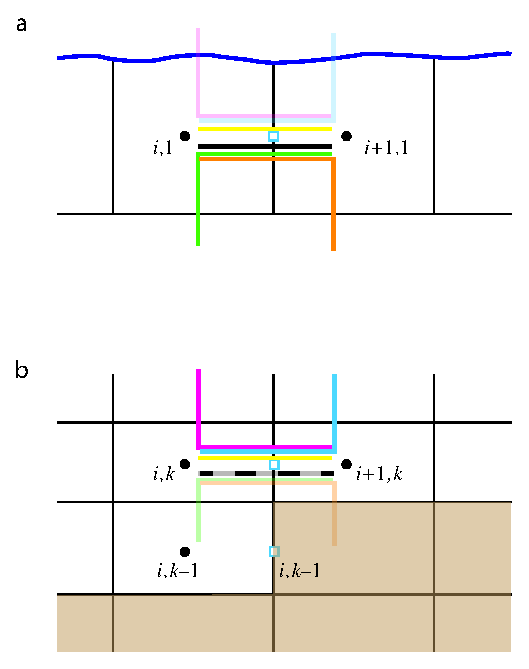
\includegraphics[width=0.60\textwidth]{Fig_GRIFF_bdry_triads}
    \caption{  \label{fig:triad:bdry_triads}
      (a) Uppermost model layer $k=1$ with $i,1$ and $i+1,1$ tracer
      points (black dots), and $i+1/2,1$ $u$-point (blue square). Triad
      slopes $\triad{i}{1}{R}{1/2}{-1/2}$ (magenta) and $\triad{i+1}{1}{R}{-1/2}{-1/2}$
      (blue) poking through the ocean surface are masked (faded in
      figure). However, the lateral $_{11}$ contributions towards
      $\triad[u]{i}{1}{F}{1/2}{-1/2}$ and $\triad[u]{i+1}{1}{F}{-1/2}{-1/2}$
      (yellow line) are still applied, giving diapycnal diffusive
      fluxes.\\
      (b) Both near bottom triad slopes $\triad{i}{k}{R}{1/2}{1/2}$ and
      $\triad{i+1}{k}{R}{-1/2}{1/2}$ are masked when either of the $i,k+1$
      or $i+1,k+1$ tracer points is masked, i.e.\ the $i,k+1$ $u$-point
      is masked. The associated lateral fluxes (grey-black dashed
      line) are masked if \np{botmix\_grif}=.false., but left
      unmasked, giving bottom mixing, if \np{botmix\_grif}=.true.}
 \end{center} \end{figure}
% >>>>>>>>>>>>>>>>>>>>>>>>>>>>
\subsection{ Limiting of the slopes within the interior}\label{sec:triad:limit}
As discussed in \S\ref{LDF_slp_iso}, iso-neutral slopes relative to
geopotentials must be bounded everywhere, both for consistency with the small-slope
approximation and for numerical stability \citep{Cox1987,
  Griffies_Bk04}. The bound chosen in \NEMO is applied to each
component of the slope separately and has a value of $1/100$ in the ocean interior.
%, ramping linearly down above 70~m depth to zero at the surface
It is of course relevant to the iso-neutral slopes $\tilde{r}_i=r_i+\sigma_i$ relative to
geopotentials (here the $\sigma_i$ are the slopes of the coordinate surfaces relative to
geopotentials) \eqref{Eq_PE_slopes_eiv} rather than the slope $r_i$ relative to coordinate
surfaces, so we require
\begin{equation*}
  |\tilde{r}_i|\leq \tilde{r}_\mathrm{max}=0.01.
\end{equation*}
and then recalculate the slopes $r_i$ relative to coordinates.
Each individual triad slope
 \begin{equation}
   \label{eq:triad:Rtilde}
_i^k\tilde{\mathbb{R}}_{i_p}^{k_p} = {}_i^k\mathbb{R}_{i_p}^{k_p}  + \frac{\delta_{i+i_p}[z_T^k]}{{e_{1u}}_{\,i + i_p}^{\,k}}
 \end{equation}
is limited like this and then the corresponding
$_i^k\mathbb{R}_{i_p}^{k_p} $ are recalculated and combined to form the fluxes.
Note that where the slopes have been limited, there is now a non-zero
iso-neutral density flux that drives dianeutral mixing.  In particular this iso-neutral density flux
is always downwards, and so acts to reduce gravitational potential energy.
\subsection{Tapering within the surface mixed layer}\label{sec:triad:taper}

Additional tapering of the iso-neutral fluxes is necessary within the
surface mixed layer. When the Griffies triads are used, we offer two
options for this.
\subsubsection{Linear slope tapering within the surface mixed layer}\label{sec:triad:lintaper}
This is the option activated by the default choice
\np{ln\_triad\_iso}=false. Slopes $\tilde{r}_i$ relative to
geopotentials are tapered linearly from their value immediately below the mixed layer to zero at the
surface, as described in option (c) of Fig.~\ref{Fig_eiv_slp}, to values
\begin{subequations}
  \begin{equation}
   \label{eq:triad:rmtilde}
     \rMLt =
  -\frac{z}{h}\left.\tilde{r}_i\right|_{z=-h}\quad \text{ for  } z>-h,
  \end{equation}
and then the $r_i$ relative to vertical coordinate surfaces are appropriately
adjusted to
  \begin{equation}
   \label{eq:triad:rm}
 \rML =\rMLt -\sigma_i \quad \text{ for  } z>-h.
  \end{equation}
\end{subequations}
Thus the diffusion operator within the mixed layer is given by:
\begin{equation} \label{eq:triad:iso_tensor_ML}
D^{lT}=\nabla {\rm {\bf .}}\left( {A^{lT}\;\Re \;\nabla T} \right) \qquad
\mbox{with}\quad \;\;\Re =\left( {{\begin{array}{*{20}c}
 1 \hfill & 0 \hfill & {-\rML[1]}\hfill \\
 0 \hfill & 1 \hfill & {-\rML[2]} \hfill \\
 {-\rML[1]}\hfill &   {-\rML[2]} \hfill & {\rML[1]^2+\rML[2]^2} \hfill
\end{array} }} \right)
\end{equation}

This slope tapering gives a natural connection between tracer in the
mixed-layer and in isopycnal layers immediately below, in the
thermocline. It is consistent with the way the $\tilde{r}_i$ are
tapered within the mixed layer (see \S\ref{sec:triad:taperskew} below)
so as to ensure a uniform GM eddy-induced velocity throughout the
mixed layer. However, it gives a downwards density flux and so acts so
as to reduce potential energy in the same way as does the slope
limiting discussed above in \S\ref{sec:triad:limit}.
 
As in \S\ref{sec:triad:limit} above, the tapering
\eqref{eq:triad:rmtilde} is applied separately to each triad
$_i^k\tilde{\mathbb{R}}_{i_p}^{k_p}$, and the
$_i^k\mathbb{R}_{i_p}^{k_p}$ adjusted. For clarity, we assume
$z$-coordinates in the following; the conversion from
$\mathbb{R}$ to $\tilde{\mathbb{R}}$ and back to $\mathbb{R}$ follows exactly as described
above by \eqref{eq:triad:Rtilde}.
\begin{enumerate}
\item Mixed-layer depth is defined so as to avoid including regions of weak
vertical stratification in the slope definition.
 At each $i,j$ (simplified to $i$ in
Fig.~\ref{fig:triad:MLB_triad}), we define the mixed-layer by setting
the vertical index of the tracer point immediately below the mixed
layer, $k_\mathrm{ML}$, as the maximum $k$ (shallowest tracer point)
such that the potential density
${\rho_0}_{i,k}>{\rho_0}_{i,k_{10}}+\Delta\rho_c$, where $i,k_{10}$ is
the tracer gridbox within which the depth reaches 10~m. See the left
side of Fig.~\ref{fig:triad:MLB_triad}. We use the $k_{10}$-gridbox
instead of the surface gridbox to avoid problems e.g.\ with thin
daytime mixed-layers. Currently we use the same
$\Delta\rho_c=0.01\;\mathrm{kg\:m^{-3}}$ for ML triad tapering as is
used to output the diagnosed mixed-layer depth
$h_\mathrm{ML}=|z_{W}|_{k_\mathrm{ML}+1/2}$, the depth of the $w$-point
above the $i,k_\mathrm{ML}$ tracer point.

\item We define `basal' triad slopes
${\:}_i{\mathbb{R}_\mathrm{base}}_{\,i_p}^{k_p}$ as the slopes
of those triads whose vertical `arms' go down from the
$i,k_\mathrm{ML}$ tracer point to the $i,k_\mathrm{ML}-1$ tracer point
below. This is to ensure that the vertical density gradients
associated with these basal triad slopes
${\:}_i{\mathbb{R}_\mathrm{base}}_{\,i_p}^{k_p}$ are
representative of the thermocline. The four basal triads defined in the bottom part
of Fig.~\ref{fig:triad:MLB_triad} are then
\begin{align}
  {\:}_i{\mathbb{R}_\mathrm{base}}_{\,i_p}^{k_p} &=
 {\:}^{k_\mathrm{ML}-k_p-1/2}_i{\mathbb{R}_\mathrm{base}}_{\,i_p}^{k_p}, \label{eq:triad:Rbase}
\\
\intertext{with e.g.\ the green triad}
{\:}_i{\mathbb{R}_\mathrm{base}}_{1/2}^{-1/2}&=
{\:}^{k_\mathrm{ML}}_i{\mathbb{R}_\mathrm{base}}_{\,1/2}^{-1/2}. \notag
\end{align}
The vertical flux associated with each of these triads passes through the $w$-point
$i,k_\mathrm{ML}-1/2$ lying \emph{below} the $i,k_\mathrm{ML}$ tracer point,
so it is this depth
\begin{equation}
  \label{eq:triad:zbase}
  {z_\mathrm{base}}_{\,i}={z_{w}}_{k_\mathrm{ML}-1/2}
\end{equation}
(one gridbox deeper than the
diagnosed ML depth $z_\mathrm{ML})$ that sets the $h$ used to taper
the slopes in \eqref{eq:triad:rmtilde}.
\item Finally, we calculate the adjusted triads
${\:}_i^k{\mathbb{R}_\mathrm{ML}}_{\,i_p}^{k_p}$ within the mixed
layer, by multiplying the appropriate
${\:}_i{\mathbb{R}_\mathrm{base}}_{\,i_p}^{k_p}$ by the ratio of
the depth of the $w$-point ${z_w}_{k+k_p}$ to ${z_\mathrm{base}}_{\,i}$. For
instance the green triad centred on $i,k$
\begin{align}
  {\:}_i^k{\mathbb{R}_\mathrm{ML}}_{\,1/2}^{-1/2} &=
\frac{{z_w}_{k-1/2}}{{z_\mathrm{base}}_{\,i}}{\:}_i{\mathbb{R}_\mathrm{base}}_{\,1/2}^{-1/2}
\notag \\
\intertext{and more generally}
 {\:}_i^k{\mathbb{R}_\mathrm{ML}}_{\,i_p}^{k_p} &=
\frac{{z_w}_{k+k_p}}{{z_\mathrm{base}}_{\,i}}{\:}_i{\mathbb{R}_\mathrm{base}}_{\,i_p}^{k_p}.\label{eq:triad:RML}
\end{align}
\end{enumerate}

% >>>>>>>>>>>>>>>>>>>>>>>>>>>>
\begin{figure}[h]
  \fcapside {\caption{\label{fig:triad:MLB_triad} Definition of
      mixed-layer depth and calculation of linearly tapered
      triads. The figure shows a water column at a given $i,j$
      (simplified to $i$), with the ocean surface at the top. Tracer points are denoted by
      bullets, and black lines the edges of the tracer cells; $k$
      increases upwards. \\
      \hspace{5 em}We define the mixed-layer by setting the vertical index
      of the tracer point immediately below the mixed layer,
      $k_\mathrm{ML}$, as the maximum $k$ (shallowest tracer point)
      such that ${\rho_0}_{i,k}>{\rho_0}_{i,k_{10}}+\Delta\rho_c$,
      where $i,k_{10}$ is the tracer gridbox within which the depth
      reaches 10~m. We calculate the triad slopes within the mixed
      layer by linearly tapering them from zero (at the surface) to
      the `basal' slopes, the slopes of the four triads passing through the
      $w$-point $i,k_\mathrm{ML}-1/2$ (blue square),
      ${\:}_i{\mathbb{R}_\mathrm{base}}_{\,i_p}^{k_p}$. Triads with
    different $i_p,k_p$, denoted by different colours, (e.g. the green
    triad $i_p=1/2,k_p=-1/2$) are tapered to the appropriate basal triad.}}
  {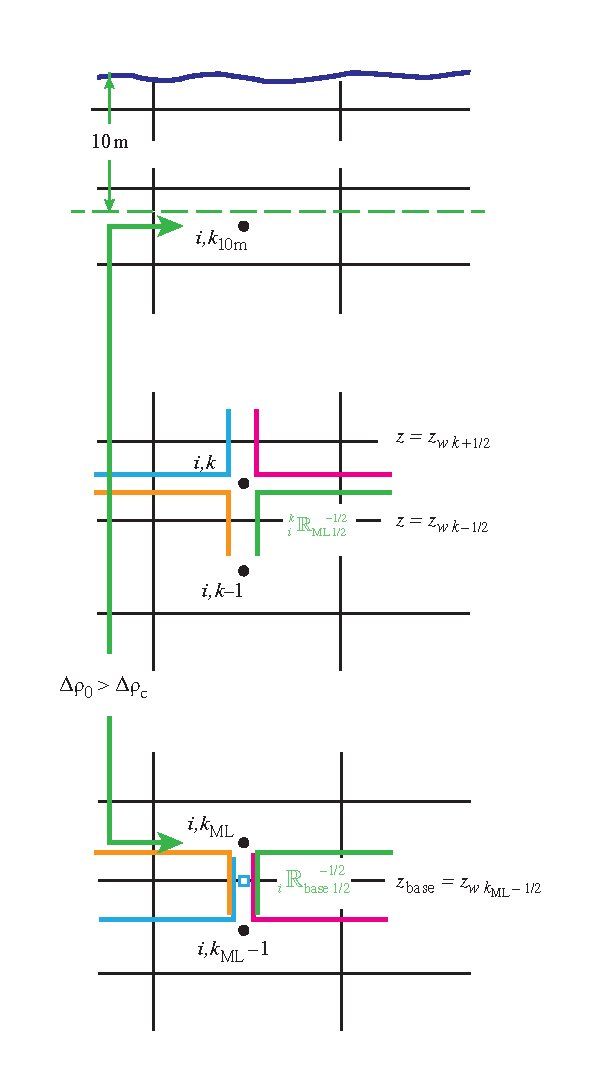
\includegraphics[width=0.60\textwidth]{Fig_GRIFF_MLB_triads}}
\end{figure}
% >>>>>>>>>>>>>>>>>>>>>>>>>>>>

\subsubsection{Additional truncation of skew iso-neutral flux
  components}
\label{sec:triad:Gerdes-taper}
The alternative option is activated by setting \np{ln\_triad\_iso} =
  true. This retains the same tapered slope $\rML$  described above for the
calculation of the $_{33}$ term of the iso-neutral diffusion tensor (the
vertical tracer flux driven by vertical tracer gradients), but
replaces the $\rML$ in the skew term by
\begin{equation}
  \label{eq:triad:rm*}
  \rML^*=\left.\rMLt^2\right/\tilde{r}_i-\sigma_i,
\end{equation}
giving a ML diffusive operator
\begin{equation} \label{eq:triad:iso_tensor_ML2}
D^{lT}=\nabla {\rm {\bf .}}\left( {A^{lT}\;\Re \;\nabla T} \right) \qquad
\mbox{with}\quad \;\;\Re =\left( {{\begin{array}{*{20}c}
 1 \hfill & 0 \hfill & {-\rML[1]^*}\hfill \\
 0 \hfill & 1 \hfill & {-\rML[2]^*} \hfill \\
 {-\rML[1]^*}\hfill &   {-\rML[2]^*} \hfill & {\rML[1]^2+\rML[2]^2} \hfill \\
\end{array} }} \right).
\end{equation}
This operator
\footnote{To ensure good behaviour where horizontal density
  gradients are weak, we in fact follow \citet{Gerdes1991} and set
$\rML^*=\mathrm{sgn}(\tilde{r}_i)\min(|\rMLt^2/\tilde{r}_i|,|\tilde{r}_i|)-\sigma_i$.}
then has the property it gives no vertical density flux, and so does
not change the potential energy.
This approach is similar to multiplying the iso-neutral  diffusion
coefficient by $\tilde{r}_\mathrm{max}^{-2}\tilde{r}_i^{-2}$ for steep
slopes, as suggested by \citet{Gerdes1991} (see also \citet{Griffies_Bk04}).
Again it is applied separately to each triad $_i^k\mathbb{R}_{i_p}^{k_p}$

In practice, this approach gives weak vertical tracer fluxes through
the mixed-layer, as well as vanishing density fluxes. While it is
theoretically advantageous that it does not change the potential
energy, it may give a discontinuity between the
fluxes within the mixed-layer (purely horizontal) and just below (along
iso-neutral surfaces).
% This may give strange looking results,
% particularly where the mixed-layer depth varies strongly laterally.
% ================================================================
% Skew flux formulation for Eddy Induced Velocity :
% ================================================================
\section{Eddy induced advection formulated as a skew flux}\label{sec:triad:skew-flux}

\subsection{The continuous skew flux formulation}\label{sec:triad:continuous-skew-flux}

 When Gent and McWilliams's [1990] diffusion is used,
an additional advection term is added. The associated velocity is the so called
eddy induced velocity, the formulation of which depends on the slopes of iso-
neutral surfaces. Contrary to the case of iso-neutral mixing, the slopes used
here are referenced to the geopotential surfaces, $i.e.$ \eqref{Eq_ldfslp_geo}
is used in $z$-coordinate, and the sum \eqref{Eq_ldfslp_geo}
+ \eqref{Eq_ldfslp_iso} in $z^*$ or $s$-coordinates.

The eddy induced velocity is given by:
\begin{subequations} \label{eq:triad:eiv}
\begin{equation}\label{eq:triad:eiv_v}
\begin{split}
 u^* & = - \frac{1}{e_{3}}\;          \partial_i\psi_1,  \\
 v^* & = - \frac{1}{e_{3}}\;          \partial_j\psi_2,    \\
w^* & =    \frac{1}{e_{1}e_{2}}\; \left\{ \partial_i  \left( e_{2} \, \psi_1\right)
							    + \partial_j  \left( e_{1} \, \psi_2\right) \right\},
\end{split}
\end{equation}
where the streamfunctions $\psi_i$ are given by
\begin{equation} \label{eq:triad:eiv_psi}
\begin{split}
\psi_1 & = A_{e} \; \tilde{r}_1,   \\
\psi_2 & = A_{e} \; \tilde{r}_2,
\end{split}
\end{equation}
\end{subequations}
with $A_{e}$ the eddy induced velocity coefficient, and $\tilde{r}_1$ and $\tilde{r}_2$ the slopes between the iso-neutral and the geopotential surfaces.

The traditional way to implement this additional advection is to add
it to the Eulerian velocity prior to computing the tracer
advection. This is implemented if \key{traldf\_eiv} is set in the
default implementation, where \np{ln\_traldf\_grif} is set
false. This allows us to take advantage of all the advection schemes
offered for the tracers (see \S\ref{TRA_adv}) and not just a $2^{nd}$
order advection scheme. This is particularly useful for passive
tracers where \emph{positivity} of the advection scheme is of
paramount importance.

However, when \np{ln\_traldf\_grif} is set true, \NEMO instead
implements eddy induced advection according to the so-called skew form
\citep{Griffies_JPO98}. It is based on a transformation of the advective fluxes
using the non-divergent nature of the eddy induced velocity.
For example in the (\textbf{i},\textbf{k}) plane, the tracer advective
fluxes per unit area in $ijk$ space can be
transformed as follows:
\begin{flalign*}
\begin{split}
\textbf{F}_\mathrm{eiv}^T =
\begin{pmatrix}
 	        {e_{2}\,e_{3}\;  u^*} 	 	\\
 		{e_{1}\,e_{2}\; w^*}	 \\
\end{pmatrix}   \;   T
&=
\begin{pmatrix}
 	        { - \partial_k \left( e_{2} \,\psi_1 \right) \; T \;} 	 	\\
 		{+ \partial_i  \left( e_{2} \, \psi_1 \right) \; T \;}	 \\
\end{pmatrix} 			\\
&=
\begin{pmatrix}
 	        { - \partial_k \left( e_{2} \, \psi_1  \; T \right) \;}  \\
 		{+ \partial_i  \left( e_{2} \,\psi_1 \; T \right) \;}	 \\
\end{pmatrix}
 +
\begin{pmatrix}
 	        {+ e_{2} \, \psi_1  \; \partial_k T}  \\
 		{ - e_{2} \, \psi_1  \; \partial_i  T}	 \\
\end{pmatrix}
\end{split}
\end{flalign*}
and since the eddy induced velocity field is non-divergent, we end up with the skew
form of the eddy induced advective fluxes per unit area in $ijk$ space:
\begin{equation} \label{eq:triad:eiv_skew_ijk}
\textbf{F}_\mathrm{eiv}^T = \begin{pmatrix}
 	        {+ e_{2} \, \psi_1  \; \partial_k T}   \\
 		{ - e_{2} \, \psi_1  \; \partial_i  T}	 \\
                                 \end{pmatrix}
\end{equation}
The total fluxes per unit physical area are then
\begin{equation}\label{eq:triad:eiv_skew_physical}
\begin{split}
 f^*_1 & = \frac{1}{e_{3}}\; \psi_1 \partial_k T   \\
 f^*_2 & = \frac{1}{e_{3}}\; \psi_2 \partial_k T   \\
 f^*_3 & =  -\frac{1}{e_{1}e_{2}}\; \left\{ e_{2} \psi_1 \partial_i T
   + e_{1} \psi_2 \partial_j T \right\}. \\
\end{split}
\end{equation}
Note that Eq.~ \eqref{eq:triad:eiv_skew_physical} takes the same form whatever the
vertical coordinate, though of course the slopes
$\tilde{r}_i$ which define the $\psi_i$ in \eqref{eq:triad:eiv_psi} are relative to geopotentials.
The tendency associated with eddy induced velocity is then simply the convergence
of the fluxes (\ref{eq:triad:eiv_skew_ijk}, \ref{eq:triad:eiv_skew_physical}), so
\begin{equation} \label{eq:triad:skew_eiv_conv}
\frac{\partial T}{\partial t}= -\frac{1}{e_1 \, e_2 \, e_3 }      \left[
  \frac{\partial}{\partial i} \left( e_2 \psi_1 \partial_k T\right)
  + \frac{\partial}{\partial j} \left( e_1  \;
    \psi_2 \partial_k T\right)
 -  \frac{\partial}{\partial k} \left( e_{2} \psi_1 \partial_i T
   + e_{1} \psi_2 \partial_j T \right)  \right]
\end{equation}
 It naturally conserves the tracer content, as it is expressed in flux
 form. Since it has the same divergence as the advective form it also
 preserves the tracer variance.

\subsection{The discrete skew flux formulation}
The skew fluxes in (\ref{eq:triad:eiv_skew_physical}, \ref{eq:triad:eiv_skew_ijk}), like the off-diagonal terms
(\ref{eq:triad:i13c}, \ref{eq:triad:i31c}) of the small angle diffusion tensor, are best
expressed in terms of the triad slopes, as in Fig.~\ref{fig:triad:ISO_triad}
and Eqs~(\ref{eq:triad:i13}, \ref{eq:triad:i31}); but now in terms of the triad slopes
$\tilde{\mathbb{R}}$ relative to geopotentials instead of the
$\mathbb{R}$ relative to coordinate surfaces. The discrete form of
\eqref{eq:triad:eiv_skew_ijk} using the slopes \eqref{eq:triad:R} and
defining $A_e$ at $T$-points is then given by:


\begin{subequations}\label{eq:triad:allskewflux}
  \begin{flalign}\label{eq:triad:vect_skew_flux}
    \vect{F}_\mathrm{eiv}(T) &\equiv
    \sum_{\substack{i_p,\,k_p}}
    \begin{pmatrix}
      {_{i+1/2-i_p}^k {\mathbb{S}_u}_{i_p}^{k_p} } (T)      \\
      \\
      {_i^{k+1/2-k_p} {\mathbb{S}_w}_{i_p}^{k_p} } (T)      \\
    \end{pmatrix},
  \end{flalign}
  where the skew flux in the $i$-direction associated with a given
  triad is (\ref{eq:triad:latflux-triad}, \ref{eq:triad:triadfluxu}):
  \begin{align}
    \label{eq:triad:skewfluxu}
    _i^k {\mathbb{S}_u}_{i_p}^{k_p} (T) &= + \quarter {A_e}_i^k{
      \:}\frac{{b_u}_{i+i_p}^k}{{e_{1u}}_{\,i + i_p}^{\,k}}
     \ {_i^k\tilde{\mathbb{R}}_{i_p}^{k_p}} \
      \frac{ \delta_{k+k_p} [T^i] }{{e_{3w}}_{\,i}^{\,k+k_p} },
   \\
    \intertext{and \eqref{eq:triad:triadfluxw} in the $k$-direction, changing the sign
      to be consistent with \eqref{eq:triad:eiv_skew_ijk}:}
    _i^k {\mathbb{S}_w}_{i_p}^{k_p} (T)
    &= -\quarter {A_e}_i^k{\: }\frac{{b_u}_{i+i_p}^k}{{e_{3w}}_{\,i}^{\,k+k_p}}
     {_i^k\tilde{\mathbb{R}}_{i_p}^{k_p}}\frac{ \delta_{i+ i_p}[T^k] }{ {e_{1u}}_{\,i + i_p}^{\,k} }.\label{eq:triad:skewfluxw}
  \end{align}
\end{subequations}

Such a discretisation is consistent with the iso-neutral
operator as it uses the same definition for the slopes.  It also
ensures the following two key properties.
\subsubsection{No change in tracer variance}
The discretization conserves tracer variance, $i.e.$ it does not
include a diffusive component but is a `pure' advection term. This can
be seen
%either from Appendix \ref{Apdx_eiv_skew} or
by considering the
fluxes associated with a given triad slope
$_i^k{\mathbb{R}}_{i_p}^{k_p} (T)$. For, following
\S\ref{sec:triad:variance} and \eqref{eq:triad:dvar_iso_i}, the
associated horizontal skew-flux $_i^k{\mathbb{S}_u}_{i_p}^{k_p} (T)$
drives a net rate of change of variance, summed over the two
$T$-points $i+i_p-\half,k$ and $i+i_p+\half,k$, of
\begin{equation}
\label{eq:triad:dvar_eiv_i}
  _i^k{\mathbb{S}_u}_{i_p}^{k_p} (T)\,\delta_{i+ i_p}[T^k],
\end{equation}
while the associated vertical skew-flux gives a variance change summed over the
$T$-points $i,k+k_p-\half$ (above) and $i,k+k_p+\half$ (below) of
\begin{equation}
\label{eq:triad:dvar_eiv_k}
  _i^k{\mathbb{S}_w}_{i_p}^{k_p} (T) \,\delta_{k+ k_p}[T^i].
\end{equation}
Inspection of the definitions (\ref{eq:triad:skewfluxu}, \ref{eq:triad:skewfluxw})
shows that these two variance changes (\ref{eq:triad:dvar_eiv_i}, \ref{eq:triad:dvar_eiv_k})
sum to zero. Hence the two fluxes associated with each triad make no
net contribution to the variance budget.

\subsubsection{Reduction in gravitational PE}
The vertical density flux associated with the vertical skew-flux
always has the same sign as the vertical density gradient; thus, so
long as the fluid is stable (the vertical density gradient is
negative) the vertical density flux is negative (downward) and hence
reduces the gravitational PE.

For the change in gravitational PE driven by the $k$-flux is
\begin{align}
  \label{eq:triad:vert_densityPE}
  g {e_{3w}}_{\,i}^{\,k+k_p}{\mathbb{S}_w}_{i_p}^{k_p} (\rho)
  &=g {e_{3w}}_{\,i}^{\,k+k_p}\left[-\alpha _i^k {\:}_i^k
    {\mathbb{S}_w}_{i_p}^{k_p} (T) + \beta_i^k {\:}_i^k
    {\mathbb{S}_w}_{i_p}^{k_p} (S) \right]. \notag \\
\intertext{Substituting  ${\:}_i^k {\mathbb{S}_w}_{i_p}^{k_p}$ from
  \eqref{eq:triad:skewfluxw}, gives}
% and separating out
% $\rtriadt{R}=\rtriad{R} + \delta_{i+i_p}[z_T^k]$,
% gives two terms. The
% first $\rtriad{R}$ term (the only term for $z$-coordinates) is:
 &=-\quarter g{A_e}_i^k{\: }{b_u}_{i+i_p}^k {_i^k\tilde{\mathbb{R}}_{i_p}^{k_p}}
\frac{ -\alpha _i^k\delta_{i+ i_p}[T^k]+ \beta_i^k\delta_{i+ i_p}[S^k]} { {e_{1u}}_{\,i + i_p}^{\,k} } \notag \\
 &=+\quarter g{A_e}_i^k{\: }{b_u}_{i+i_p}^k
     \left({_i^k\mathbb{R}_{i_p}^{k_p}}+\frac{\delta_{i+i_p}[z_T^k]}{{e_{1u}}_{\,i + i_p}^{\,k}}\right) {_i^k\mathbb{R}_{i_p}^{k_p}}
\frac{-\alpha_i^k \delta_{k+ k_p}[T^i]+ \beta_i^k\delta_{k+ k_p}[S^i]} {{e_{3w}}_{\,i}^{\,k+k_p}},
\end{align}
using the definition of the triad slope $\rtriad{R}$,
\eqref{eq:triad:R} to express $-\alpha _i^k\delta_{i+ i_p}[T^k]+
\beta_i^k\delta_{i+ i_p}[S^k]$ in terms of  $-\alpha_i^k \delta_{k+
  k_p}[T^i]+ \beta_i^k\delta_{k+ k_p}[S^i]$.

Where the coordinates slope, the $i$-flux gives a PE change
\begin{multline}
  \label{eq:triad:lat_densityPE}
 g \delta_{i+i_p}[z_T^k]
\left[
-\alpha _i^k {\:}_i^k {\mathbb{S}_u}_{i_p}^{k_p} (T) + \beta_i^k {\:}_i^k {\mathbb{S}_u}_{i_p}^{k_p} (S)
\right] \\
= +\quarter g{A_e}_i^k{\: }{b_u}_{i+i_p}^k
     \frac{\delta_{i+i_p}[z_T^k]}{{e_{1u}}_{\,i + i_p}^{\,k}}
\left({_i^k\mathbb{R}_{i_p}^{k_p}}+\frac{\delta_{i+i_p}[z_T^k]}{{e_{1u}}_{\,i + i_p}^{\,k}}\right)
\frac{-\alpha_i^k \delta_{k+ k_p}[T^i]+ \beta_i^k\delta_{k+ k_p}[S^i]} {{e_{3w}}_{\,i}^{\,k+k_p}},
\end{multline}
(using \eqref{eq:triad:skewfluxu}) and so the total PE change
\eqref{eq:triad:vert_densityPE} + \eqref{eq:triad:lat_densityPE} associated with the triad fluxes is
\begin{multline}
  \label{eq:triad:tot_densityPE}
  g{e_{3w}}_{\,i}^{\,k+k_p}{\mathbb{S}_w}_{i_p}^{k_p} (\rho) +
g\delta_{i+i_p}[z_T^k] {\:}_i^k {\mathbb{S}_u}_{i_p}^{k_p} (\rho) \\
= +\quarter g{A_e}_i^k{\: }{b_u}_{i+i_p}^k
     \left({_i^k\mathbb{R}_{i_p}^{k_p}}+\frac{\delta_{i+i_p}[z_T^k]}{{e_{1u}}_{\,i + i_p}^{\,k}}\right)^2
\frac{-\alpha_i^k \delta_{k+ k_p}[T^i]+ \beta_i^k\delta_{k+ k_p}[S^i]} {{e_{3w}}_{\,i}^{\,k+k_p}}.
\end{multline}
Where the fluid is stable, with $-\alpha_i^k \delta_{k+ k_p}[T^i]+
\beta_i^k\delta_{k+ k_p}[S^i]<0$, this PE change is negative.

\subsection{Treatment of the triads at the boundaries}\label{sec:triad:skew_bdry}
Triad slopes \rtriadt{R} used for the calculation of the eddy-induced skew-fluxes
are masked at the boundaries in exactly the same way as are the triad
slopes \rtriad{R} used for the iso-neutral diffusive fluxes, as
described in \S\ref{sec:triad:iso_bdry} and
Fig.~\ref{fig:triad:bdry_triads}. Thus surface layer triads
$\triadt{i}{1}{R}{1/2}{-1/2}$ and $\triadt{i+1}{1}{R}{-1/2}{-1/2}$ are
masked, and both near bottom triad slopes $\triadt{i}{k}{R}{1/2}{1/2}$
and $\triadt{i+1}{k}{R}{-1/2}{1/2}$ are masked when either of the
$i,k+1$ or $i+1,k+1$ tracer points is masked, i.e.\ the $i,k+1$
$u$-point is masked. The namelist parameter \np{ln\_botmix\_grif} has
no effect on the eddy-induced skew-fluxes.

\subsection{ Limiting of the slopes within the interior}\label{sec:triad:limitskew}
Presently, the iso-neutral slopes $\tilde{r}_i$ relative
to geopotentials are limited to be less than $1/100$, exactly as in
calculating the iso-neutral diffusion, \S \ref{sec:triad:limit}. Each
individual triad \rtriadt{R} is so limited.

\subsection{Tapering within the surface mixed layer}\label{sec:triad:taperskew}
The slopes $\tilde{r}_i$ relative to
geopotentials (and thus the individual triads \rtriadt{R}) are always tapered linearly from their value immediately below the mixed layer to zero at the
surface \eqref{eq:triad:rmtilde}, as described in \S\ref{sec:triad:lintaper}. This is
option (c) of Fig.~\ref{Fig_eiv_slp}. This linear tapering for the
slopes used to calculate the eddy-induced fluxes is
unaffected by the value of \np{ln\_triad\_iso}.

The justification for this linear slope tapering is that, for $A_e$
that is constant or varies only in the horizontal (the most commonly
used options in \NEMO: see \S\ref{LDF_coef}), it is
equivalent to a horizontal eiv (eddy-induced velocity) that is uniform
within the mixed layer \eqref{eq:triad:eiv_v}. This ensures that the
eiv velocities do not restratify the mixed layer \citep{Treguier1997,
  Danabasoglu_al_2008}. Equivantly, in terms
of the skew-flux formulation we use here, the
linear slope tapering within the mixed-layer gives a linearly varying
vertical flux, and so a tracer convergence uniform in depth (the
horizontal flux convergence is relatively insignificant within the mixed-layer).

\subsection{Streamfunction diagnostics}\label{sec:triad:sfdiag}
Where the namelist parameter \np{ln\_traldf\_gdia}=true, diagnosed
mean eddy-induced velocities are output. Each time step,
streamfunctions are calculated in the $i$-$k$ and $j$-$k$ planes at
$uw$ (integer +1/2 $i$, integer $j$, integer +1/2 $k$) and $vw$
(integer $i$, integer +1/2 $j$, integer +1/2 $k$) points (see Table
\ref{Tab_cell}) respectively. We follow \citep{Griffies_Bk04} and
calculate the streamfunction at a given $uw$-point from the
surrounding four triads according to:
\begin{equation}
  \label{eq:triad:sfdiagi}
  {\psi_1}_{i+1/2}^{k+1/2}={\quarter}\sum_{\substack{i_p,\,k_p}}
  {A_e}_{i+1/2-i_p}^{k+1/2-k_p}\:\triadd{i+1/2-i_p}{k+1/2-k_p}{R}{i_p}{k_p}.
\end{equation}
The streamfunction $\psi_1$ is calculated similarly at $vw$ points.
The eddy-induced velocities are then calculated from the
straightforward discretisation of \eqref{eq:triad:eiv_v}:
\begin{equation}\label{eq:triad:eiv_v_discrete}
\begin{split}
 {u^*}_{i+1/2}^{k} & = - \frac{1}{{e_{3u}}_{i}^{k}}\left({\psi_1}_{i+1/2}^{k+1/2}-{\psi_1}_{i+1/2}^{k+1/2}\right),   \\
 {v^*}_{j+1/2}^{k} & = - \frac{1}{{e_{3v}}_{j}^{k}}\left({\psi_2}_{j+1/2}^{k+1/2}-{\psi_2}_{j+1/2}^{k+1/2}\right),   \\
 {w^*}_{i,j}^{k+1/2} & =    \frac{1}{e_{1t}e_{2t}}\; \left\{
 {e_{2u}}_{i+1/2}^{k+1/2} \,{\psi_1}_{i+1/2}^{k+1/2} -
 {e_{2u}}_{i-1/2}^{k+1/2} \,{\psi_1}_{i-1/2}^{k+1/2} \right. + \\
\phantom{=} & \qquad\qquad\left. {e_{2v}}_{j+1/2}^{k+1/2} \,{\psi_2}_{j+1/2}^{k+1/2} - {e_{2v}}_{j-1/2}^{k+1/2} \,{\psi_2}_{j-1/2}^{k+1/2} \right\},
\end{split}
\end{equation}
\end{document}
